\documentclass[conference]{IEEEtran}
\IEEEoverridecommandlockouts
\usepackage{cite}
\usepackage{amsmath,amssymb,amsfonts}
\usepackage{algorithmic}
\usepackage{graphicx}
\usepackage{textcomp}
\usepackage{xcolor}
\usepackage{threeparttable}
\usepackage{float}
\usepackage{hyperref}

\floatstyle{boxed} 
\restylefloat{figure}

\def\BibTeX{{\rm B\kern-.05em{\sc i\kern-.025em b}\kern-.08em
    T\kern-.1667em\lower.7ex\hbox{E}\kern-.125emX}}
\begin{document}

\title{Sleep State Prediction Using Accelerometry Data: A Systematic and Computational Approach}

\author{
	\IEEEauthorblockN{Juan Carlos Quintero Rubiano}
	\IEEEauthorblockA{Code: 20232020172\\
		\textit{Systems Engineering} \\
		\textit{Francisco Jose de Caldas District University}\\
		Bogota, Colombia \\
		jcquineror@udistrital.edu.co}\\
	%and
	\IEEEauthorblockN{Juan Felipe Wilches Gomez}
	\IEEEauthorblockA{Code: 20231020137\\
		\textit{Systems Engineering} \\
		\textit{Francisco Jose de Caldas District University}\\
		Bogota, Colombia \\
		jfwilchesg@udistrital.edu.co}
	\and
	\IEEEauthorblockN{Juan Nicolas Diaz Salamanca}
	\IEEEauthorblockA{Code: 20232020059\\
		\textit{Systems Engineering} \\
		\textit{Francisco Jose de Caldas District University}\\
		Bogota, Colombia \\
		jndiazs@udistrital.edu.co}
}

\maketitle
\begin{abstract}
	Sleep constitutes a fundamental physiological process comprising multiple distinct states, each fulfilling critical roles in maintaining optimal health and cognitive function. As a highly sensitive biological system, sleep demonstrates exceptional susceptibility to environmental perturbations, whereby subtle variations in ambient conditions, acoustic environments, or external stimuli can substantially influence sleep onset latency, duration, and state transition quality. Conventional sleep state assessment relies predominantly on polysomnography (PSG), a methodology that is both financially prohibitive and clinically intrusive. Contemporary advances in wearable sensor technology have facilitated the utilization of accelerometric devices as non-invasive, cost-effective alternatives for sleep state prediction. This investigation presents a comprehensive systematic analysis and computational framework for predicting sleep states through accelerometric data analysis, emphasizing the extraction of movement patterns and temporal characteristics while accounting for the inherent environmental sensitivity of sleep systems. We examine the theoretical foundations, computational models, and methodological considerations, elucidating both the potential and limitations of accelerometer-based sleep monitoring in capturing environmentally-influenced state transitions.
\end{abstract}

\begin{IEEEkeywords}
	Sleep state classification, accelerometry, computational modeling, wearable sensing technologies, circadian rhythm analysis, temporal feature extraction.
\end{IEEEkeywords}

\section{Introduction}

Sleep represents a fundamental biological process that exerts profound influence on physical health, cognitive performance, and psychological well-being \cite{walker2017we}. Conventional sleep state assessment relies predominantly on polysomnography (PSG), which necessitates simultaneous recording of multiple physiological signals including electroencephalography (EEG), electrooculography (EOG), and electromyography (EMG) \cite{berry2012rules}. However, PSG requires specialized facilities, trained technicians, and sophisticated instrumentation, rendering it financially prohibitive and geographically inaccessible for widespread clinical applications \cite{sadeh2011role}.

The proliferation of wearable sensor technology has facilitated continuous sleep monitoring through actigraphic approaches, which employ accelerometric sensors to quantify movement patterns \cite{ancoli2003role}. The foundational principle establishes that sleep epochs are characterized by markedly reduced motor activity, whereas wake periods demonstrate substantially increased movement amplitude. Contemporary tri-axial accelerometers capture high-resolution acceleration data across three spatial dimensions, providing comprehensive information for robust sleep state inference.

Actigraphy has established itself as a cornerstone technology for non-invasive sleep monitoring, with extensive research validating its effectiveness across diverse populations \cite{smith2018use}. Traditional actigraphic algorithms have dominated the field for decades, with the Cole-Kripke algorithm introducing a weighted scoring system that incorporates current epoch activity and surrounding temporal context \cite{cole1992automatic}. This algorithm demonstrates robust performance in healthy adults, achieving 85-90% accuracy when validated against polysomnography. Concurrently, the Sadeh algorithm represents another foundational approach, originally designed for pediatric populations but adapted for adult applications \cite{sadeh1994activity}. The Sadeh methodology employs different weighting schemes and incorporates variability measures across adjacent epochs \cite{meltzer2012direct}.

Contemporary developments have introduced sophisticated approaches transcending traditional activity counting paradigms. The OPAL algorithm represents significant advancement by incorporating postural information alongside activity metrics \cite{hickey2021smart}. Machine learning methodologies have been progressively applied to actigraphic data, demonstrating substantial accuracy improvements through feature engineering and ensemble approaches \cite{beattie2017estimation}. Recent advances in artificial intelligence have demonstrated the potential of Large Language Models (LLMs) for time series analysis applications, exhibiting remarkable capabilities in pattern recognition and temporal sequence modeling that translate to physiological signal analysis \cite{jin2023time}. The attention mechanisms in transformer architectures enable capture of long-range temporal dependencies, particularly relevant for circadian rhythm analysis \cite{zhou2023onellm}.

Comprehensive evaluations reveal substantial variations in classification performance across different populations and sleep conditions \cite{martin2011wrist}. The Cole-Kripke algorithm typically demonstrates superior performance in healthy adults with regular sleep patterns, while the Sadeh algorithm shows better sensitivity for detecting sleep fragmentation \cite{cellini2013direct}. Contemporary research emphasizes the importance of personalized algorithm calibration, recognizing that individual differences significantly impact classification accuracy \cite{koesmahargyo2019accuracy}.

This investigation presents a systematic computational approach for predicting sleep states utilizing accelerometric data from wearable devices. Our framework encompasses comprehensive data preprocessing, sophisticated feature extraction, and application of both traditional and contemporary computational models for sleep-wake classification, providing a comprehensive framework for accelerometer-based sleep state prediction.

\section{Method and Materials}

The development of our sleep state prediction system followed a systematic three-phase approach, beginning with comprehensive system analysis, followed by architectural design, and culminating in behavioral simulation studies. This methodology ensured a thorough understanding of the problem domain while establishing robust technical foundations for the proposed solution.

During the initial workshop phase, we conducted an extensive systems analysis to identify the fundamental components and interactions within sleep monitoring ecosystems. This analysis revealed the complex interplay between physiological signals, environmental factors, and technological constraints that characterize sleep state detection systems. We identified several sources of chaos and uncertainty within traditional sleep monitoring approaches, including signal artifacts from movement, environmental perturbations affecting sleep quality, and the inherent variability in individual sleep patterns. The systems perspective highlighted the need for adaptive algorithms capable of handling these dynamic interactions while maintaining classification accuracy across diverse populations and conditions.

\begin{figure}[htbp]
\centering
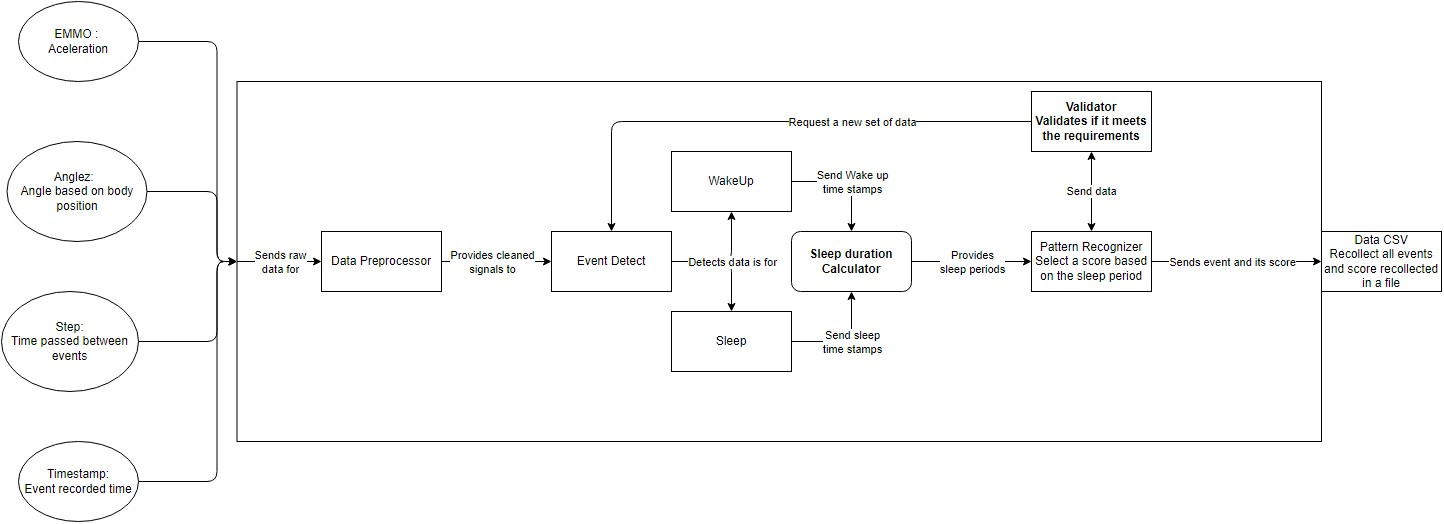
\includegraphics[width=\columnwidth]{system_analysis_workshop1.png}
\caption{Initial systems analysis from Workshop 1 showing the identification of key components, data flows, and processing stages in the sleep monitoring ecosystem, including validation mechanisms and pattern recognition elements.}
\label{fig:workshop1_analysis}
\end{figure}

The second workshop phase focused on architectural selection and system design, where we evaluated multiple computational architectures before selecting a modular approach as the most suitable solution for our problem domain. The modular architecture was chosen due to its inherent flexibility, scalability, and maintainability advantages over monolithic approaches. This architecture enables independent development and optimization of individual components while facilitating seamless integration and data flow between modules. The modular design also supports future enhancements and algorithm substitutions without requiring complete system redesign, making it particularly suitable for research and development environments where iterative improvements are essential.

Our proposed system architecture comprises five interconnected modules that collectively address the sleep state prediction challenge. The Data Acquisition module handles the collection and initial processing of accelerometric data from wearable devices, incorporating timestamp synchronization and basic quality assessment protocols. The Data Processing module performs signal calibration, normalization, filtering, and gap detection to ensure data integrity and consistency. The Feature Extraction module implements sophisticated algorithms to extract meaningful temporal and frequency domain characteristics from the preprocessed signals, including activity counts, time patterns, and statistical measures that characterize movement behaviors during different sleep states.

The Classification module represents the core intelligence of the system, implementing multiple algorithmic approaches including traditional methods such as Cole-Kripke and Sadeh algorithms, alongside contemporary machine learning techniques. This module reduces input data complexity while maintaining essential discriminative information for accurate sleep state determination. Finally, the Sleep State Prediction module integrates classification results with temporal sequence analysis to generate robust sleep state predictions, incorporating validation mechanisms to ensure prediction quality and reliability.

The third workshop phase involved comprehensive behavioral simulation studies designed to understand how external factors influence sleep patterns and system performance. These simulations examined the impact of environmental variables such as ambient noise, lighting conditions, and temperature fluctuations on sleep onset, duration, and quality transitions. The simulation framework enabled systematic evaluation of algorithm robustness under various perturbation scenarios, providing insights into system limitations and optimization opportunities. These studies revealed that environmental sensitivity varies significantly across individuals and sleep stages, reinforcing the importance of adaptive algorithmic approaches that can accommodate these variations.

The modular architecture facilitates independent validation and optimization of each component while ensuring seamless data flow and processing efficiency. Each module incorporates error handling and quality assessment mechanisms to maintain system reliability and provide transparency in the prediction process. The design enables real-time processing capabilities while supporting offline analysis for research applications, making it suitable for both clinical and consumer-oriented implementations.

\begin{figure}[htbp]
\centering
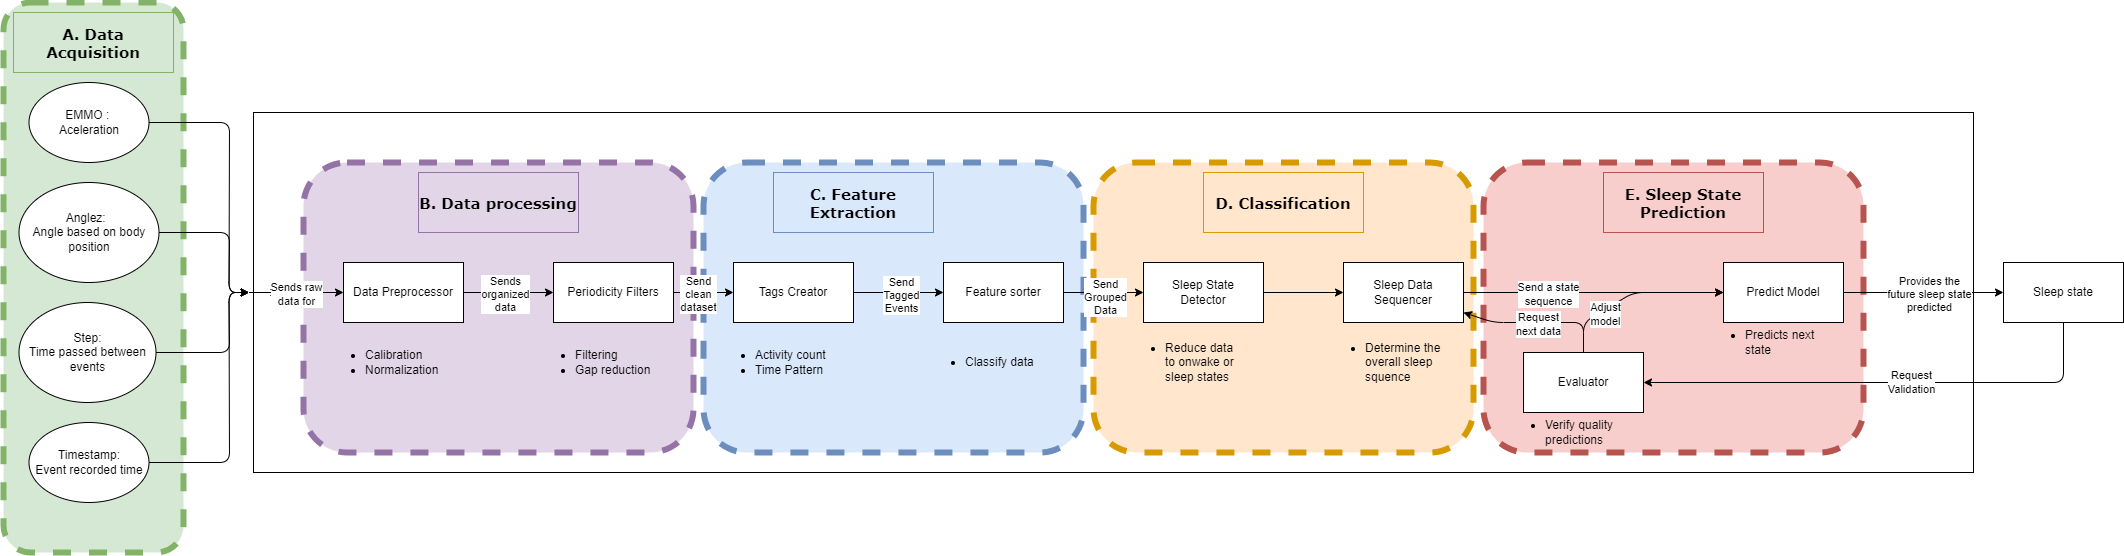
\includegraphics[width=\columnwidth]{system_architecture.png}
\caption{Modular architecture for sleep state prediction system showing the five interconnected modules: Data Acquisition, Data Processing, Feature Extraction, Classification, and Sleep State Prediction.}
\label{fig:architecture}
\end{figure}

\bibliographystyle{IEEEtran}
\bibliography{references}

\end{document}